\documentclass{beamer}
\usepackage[utf8]{inputenc}
\usepackage{bm}
\usepackage{tikz}
\usepackage{amsmath}
\usetikzlibrary{arrows}

\usetheme{Madrid}
\usecolortheme{default}


%------------------------------------------------------------
%This block of code defines the information to appear in the
%Title page
\title[Cluster Point] %optional
{Cluster Point}

% \subtitle{A short story}

\author[H.~Han]
{H.~Han}

% \institute[VFU] % (optional)
% {
%   \inst{1}%
%   Faculty of Physics\\
%   Very Famous University
%   \and
%   \inst{2}%
%   Faculty of Chemistry\\
%   Very Famous University
% }

% \date[VLC 2021] % (optional)
% {Very Large Conference, April 2021}


%End of title page configuration block
%------------------------------------------------------------



%------------------------------------------------------------
%The next block of commands puts the table of contents at the 
%beginning of each section and highlights the current section:

% \AtBeginSection[]
% {
%   \begin{frame}
%     \frametitle{Table of Contents}
%     \tableofcontents[currentsection]
%   \end{frame}
% }
%------------------------------------------------------------


\begin{document}

%The next statement creates the title page.
\frame{\titlepage}


%---------------------------------------------------------
%This block of code is for the table of contents after
%the title page
% \begin{frame}
% \frametitle{Table of Contents}
% \tableofcontents
% \end{frame}
%---------------------------------------------------------


\section{First section}

%---------------------------------------------------------
%Changing visivility of the text
% \begin{frame}
% \frametitle{Sample frame title}
% This is a text in second frame. For the sake of showing an example.
%
% \begin{itemize}
%     \item<1-> Text visible on slide 1
%     \item<2-> Text visible on slide 2
%     \item<3> Text visible on slides 3
%     \item<4-> Text visible on slide 4
% \end{itemize}
% \end{frame}

%---------------------------------------------------------


%---------------------------------------------------------
%Example of the \pause command
% \begin{frame}
% In this slide \pause
%
% the text will be partially visible \pause
%
% And finally everything will be there
% \end{frame}
%---------------------------------------------------------

% \section{Second section}

%---------------------------------------------------------
\begin{frame}
\frametitle{Open Balls}

\begin{block}{Open Balls in $\mathbb{R}^n$}
	Let $\bm{a}$ be a point in $\mathbb{R}^n$ and $r$ be a positive real number. The open ball of radius $r$ centered at $\bm{a}$ is the set 
	$$B(\bm{a}, r) = \{\bm{x} \in \mathbb{R}^n: \|\bm{x} - \bm{a}\| < r\}$$
\end{block}

\begin{examples}
	In $\mathbb{R}$, $B(\bm{1}, 1) \equiv (0,2)$
\begin{figure}
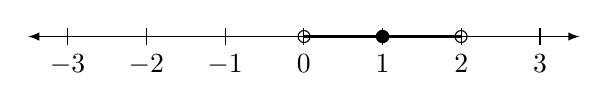
\begin{tikzpicture}
\centering
\draw[latex-latex] (-3.5,0) -- (3.5,0) ; %edit here for the axis
\foreach \x in  {-3,-2,-1,0,1,2,3} % edit here for the vertical lines
\draw[shift={(\x,0)},color=black] (0pt,3pt) -- (0pt,-3pt);
\foreach \x in {-3,-2,-1,0,1,2,3} % edit here for the numbers
\draw[shift={(\x,0)},color=black] (0pt,0pt) -- (0pt,-3pt) node[below] 
{$\x$};

\draw[*-o] (0.92,0) -- (2.08,0);
\draw[o-o] (-0.08,0) -- (1.08,0);
\draw[very thick] (1,0) -- (2,0);
\draw[very thick] (0.00,0) -- (1.00,0);
\end{tikzpicture}
\end{figure}
\end{examples}


% \begin{alertblock}{Important theorem}
% Sample text in red box
% \end{alertblock}
%
% \begin{examples}
% Sample text in green box. The title of the block is ``Examples".
% \end{examples}
\end{frame}

\begin{frame}
\frametitle{Cluster Point}
Intuitively: around it there are infinitely many other points.
\begin{block}{Accumulation Point}
	Let $S$ be a subset of $\mathbb{R}^n$. 
	$\bm{a}$ is accumulation point of $S$ if every open ball centered at $\bm{a}$ contain at least one other point in $S$ that is not $\bm{a}$.
\end{block}

No direct reference to infinity: but sufficient: there are infinitely many points in any open ball centered at $\bm{a}$.

\begin{block}{Proof}
	Say in an open ball centered at $a$ there are only finitely many points in $S$. 
	Let the distance between $\bm{a}$ and the closest point to it be $r$.
There is no points in $S$ in $B(\bm{a},r)$

\begin{figure}
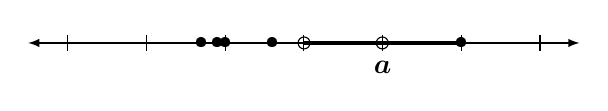
\begin{tikzpicture}
\centering
\draw[latex-latex] (-3.5,0) -- (3.5,0) ; %edit here for the axis
\foreach \x in  {-3,-2,-1,0,1,2,3} % edit here for the vertical lines
\draw[shift={(\x,0)},color=black] (0pt,3pt) -- (0pt,-3pt);

% draw a
\draw[shift={(1,0)}] (0pt,0pt) -- (0pt,-3pt) node[below] 
{$\bm{a}$};

\foreach \Point in {(2,0), (-1,0), (-1.3,0), (-1.1,0), (-0.4,0)}{
    \node at \Point {\textbullet};
	}

\draw[o-o] (-0.08,0) -- (1.08,0);
\draw[very thick] (1,0) -- (2,0);
\draw[very thick] (0.00,0) -- (1.00,0);
\end{tikzpicture}
\end{figure}
\end{block}
\end{frame}

\begin{frame}
\frametitle{Close Set}

\begin{block}{Closed Set}
	Let $S$ be a subset of $\mathbb{R}^n$. 
	$S$ is closed if it contains all its accumulation points.
\end{block}

\begin{examples}
	\begin{enumerate}
		\item $S = \{a, b, c \cdots|a,b,c \cdots \in \mathbb{R}^n\}$ is closed.
		\item $[a,b]$ is closed.
	\end{enumerate}
\end{examples}

\begin{block}{ Open Set } 
	A set is open if its complement is closed.
\end{block}

\end{frame}

%---------------------------------------------------------
%Two columns
% \begin{frame}
% \frametitle{Two-column slide}
%
% \begin{columns}
%
% \column{0.5\textwidth}
% This is a text in first column.
% $$E=mc^2$$
% \begin{itemize}
% \item First item
% \item Second item
% \end{itemize}
%
% \column{0.5\textwidth}
% This text will be in the second column
% and on a second tought this is a nice looking
% layout in some cases.
% \end{columns}
% \end{frame}
%---------------------------------------------------------


\end{document}
